\documentclass[a4paper, 12pt]{article}

\usepackage{cmap} % поиск в PDF l

\usepackage[utf8]{inputenc} % кодировка исходного текста
\usepackage[T2A]{fontenc}
\usepackage[english,russian]{babel} % локализация и переносы
\usepackage{amsmath, amsfonts, amssymb, amsthm,mathtools, float}
\usepackage{ stmaryrd }

% Рисунки
\usepackage{graphicx}
\usepackage{wrapfig}

\usepackage[left=2cm,right=2cm, top=2cm,bottom=2cm,bindingoffset=0cm]{geometry}

\usepackage{longtable}
\graphicspath{pictures}

\author{Балдин Виктор Б01-303}
\title{Работа 1.1.4 \\ Измерение интенсивности радиационного фона}

\begin{document}

	\maketitle
	\section{Аннотация}
	\textbf{Цель работы:} применение методов обработки экспериментальных данных
	для изучения статистических закономерностей
	при измерении интенсивности радиационного фона.
	\bigskip\\
	\textbf{Оборудование:} счетчик Гейгера-Мюллера (CTC-6), блок питания, компьютер
	с интерфейсом связи со счетчиком.

	\section{Теоретические сведения}
	В данной работе измеряется число частиц, проходящих через счетчик за 10 секунд, с помощью которого мы можем найти и количество за 40 секунд. Такие времена выбраны для того, чтобы показать, что при большем времени лучше выполняется нормальное распределение измеряемых величин и гистограмма более симметрична, чем при малых временах, когда при обработке лучше воспользоваться законом Пуассона.

	Если случайные события, такие как регистрация частицы счётчиком, однородны во времени и являются независимыми, то результаты их измерений подчиняются распределению Пуассона. Теория вероятности утверждает, что в таком случае:
	\begin{equation}
		\sigma = \sqrt{n_0}
	\end{equation}


		Для рассмотренной выборки из $n$ измерений относительная ошибка отдельного измерения равна:
	\begin{equation}
		\varepsilon_{\mbox{\tiny{отд}}} \approx \frac{1}{\sqrt{n_i}}
	\end{equation}
	При проведении многочисленных опытов за $n_0$ принимается среднее арифметическое всех результатов
	$\langle n \rangle$, а стандартное отклонение $\langle n \rangle$ от $n_0$ может быть
	вычислено по формуле:
	\[ \sigma_{\langle n \rangle} = \frac{1}{N} \sqrt{\sum_{i=1}^N(n_i - \langle n \rangle)^2}, \] где $N$ - количество измерений, $n_i$ - результат $i$-того измерения. Относительная же погрешность составит: \[ \varepsilon_{\langle n \rangle} = \frac{1}{\sqrt{\langle n \rangle N}}. \]
	Таким образом, можно по результатам измерений можно построить гистограмму $\omega_n = f(n)$, где $\omega_n
	$ -- доля случаев, для которых число срабатывания счетчика за 10 с равно $n$.

 	\section{Методика измерений}
	\begin{figure}[H]
		\centering
		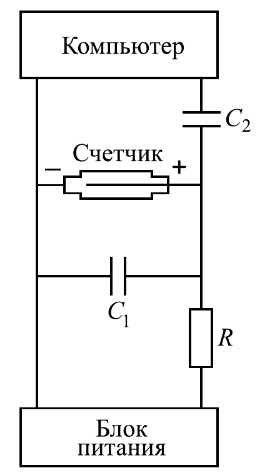
\includegraphics[scale = 0.5]{pictures/scheme.png}
		\caption{Схема включения датчика}
	\end{figure}

	Космические лучи обнаруживают с помощью ионизации, которую они производят, используя счетчик Гейгера-Мюллера. Схема его подключения приведена на рисунке 1. Счетчик представляет собой наполненный газом сосуд с двумя электродами. Частицы космических лчей ионизируют газ, выбивают электроны из стенок сосуда. Те, сталкиваясь с молекулами газа, выбивают из них электроны. Таким образом, получается лавина электронов, вследствие которой через счетчик резко увеличивается сила тока.

	\section{Используемое оборудование}
	Счетчик Гейгера-Мюллера (СТС-6), блок питания, компьютер.

	\section{Результаты измерений и обработка данных}

	\begin{enumerate}
		\item Включим установку и убедимся в ее работоспособности, проведя демонстрационный
		эксперимент.
		\item Проведем основной эксперимент. Данные, полученные для количества частиц,
		прошедших за 20 с:
		\begin{table}[H]
			\centering
			\caption{Количество срабатываний за 20 с}
			\begin{tabular}{|c|c|c|c|c|c|c|c|c|c|c|}
			\hline
			№ опыта & 1  & 2  & 3  & 4  & 5  & 6  & 7  & 8  & 9  & 10 \\ \hline
			0       & 31 & 25 & 24 & 19 & 24 & 19 & 27 & 27 & 22 & 25 \\ \hline
			10      & 23 & 37 & 36 & 25 & 25 & 22 & 28 & 24 & 23 & 29 \\ \hline
			20      & 24 & 21 & 28 & 28 & 24 & 24 & 28 & 25 & 27 & 30 \\ \hline
			30      & 23 & 29 & 26 & 36 & 21 & 35 & 23 & 20 & 34 & 24 \\ \hline
			40      & 22 & 19 & 34 & 22 & 30 & 30 & 20 & 32 & 33 & 20 \\ \hline
			50      & 28 & 28 & 21 & 25 & 35 & 18 & 26 & 22 & 24 & 26 \\ \hline
			60      & 16 & 27 & 26 & 24 & 27 & 19 & 31 & 15 & 28 & 38 \\ \hline
			70      & 24 & 33 & 24 & 29 & 31 & 21 & 15 & 20 & 26 & 19 \\ \hline
			80      & 20 & 18 & 41 & 25 & 22 & 24 & 22 & 21 & 30 & 25 \\ \hline
			90      & 20 & 31 & 31 & 24 & 14 & 19 & 29 & 17 & 14 & 28 \\ \hline
			100     & 25 & 31 & 29 & 29 & 18 & 25 & 18 & 24 & 24 & 35 \\ \hline
			110     & 31 & 21 & 31 & 32 & 34 & 13 & 29 & 30 & 21 & 20 \\ \hline
			120     & 30 & 22 & 20 & 32 & 32 & 29 & 33 & 20 & 31 & 29 \\ \hline
			130     & 26 & 18 & 22 & 29 & 33 & 20 & 33 & 20 & 31 & 29 \\ \hline
			140     & 22 & 25 & 27 & 23 & 18 & 28 & 21 & 23 & 24 & 27 \\ \hline
			150     & 27 & 25 & 30 & 21 & 24 & 23 & 22 & 33 & 21 & 32 \\ \hline
			160     & 28 & 22 & 26 & 20 & 31 & 29 & 30 & 27 & 23 & 26 \\ \hline
			170     & 22 & 24 & 20 & 31 & 38 & 18 & 24 & 28 & 26 & 24 \\ \hline
			180     & 41 & 28 & 27 & 29 & 25 & 23 & 21 & 24 & 26 & 19 \\ \hline
			190     & 27 & 24 & 25 & 34 & 28 & 28 & 19 & 28 & 26 & 21 \\ \hline
			\end{tabular}
		\end{table}

		\item Переносим данные для $\tau = 10$ с:
		\begin{table}[H]
			\centering
			\caption{Данные для гистограммы для $\tau = 10$ с}
			\begin{tabular}{|c|c|c|}
			\hline
			Число импульсов $n$ & Число случаев & Доля случаев $\omega_n$  \\ \hline
			4                   & 4             & 0.0100                   \\ \hline
			5                   & 1             & 0.0025                   \\ \hline
			6                   & 9             & 0.0225                   \\ \hline
			7                   & 20            & 0.0500                   \\ \hline
			8                   & 19            & 0.0475                   \\ \hline
			9                   & 25            & 0.0625                   \\ \hline
			10                  & 39            & 0.0975                   \\ \hline
			11                  & 33            & 0.0825                   \\ \hline
			12                  & 41            & 0.1025                   \\ \hline
			13                  & 43            & 0.1075                   \\ \hline
			14                  & 47            & 0.1175                   \\ \hline
			15                  & 36            & 0.0900                   \\ \hline
			16                  & 23            & 0.0575                   \\ \hline
			17                  & 11            & 0.0275                   \\ \hline
			18                  & 27            & 0.0675                   \\ \hline
			19                  & 6             & 0.0150                   \\ \hline
			20                  & 6             & 0.0150                   \\ \hline
			21                  & 3             & 0.0075                   \\ \hline
			22                  & 2             & 0.0050                   \\ \hline
			23                  & 4             & 0.0100                   \\ \hline
			27                  & 1             & 0.0025                   \\ \hline
			\end{tabular}
		\end{table}

		\item Построим гистограмму по таблице 2:
		\begin{figure}[H]
			\centering
			\caption{Гистограмма для $\tau = 10$ с}
			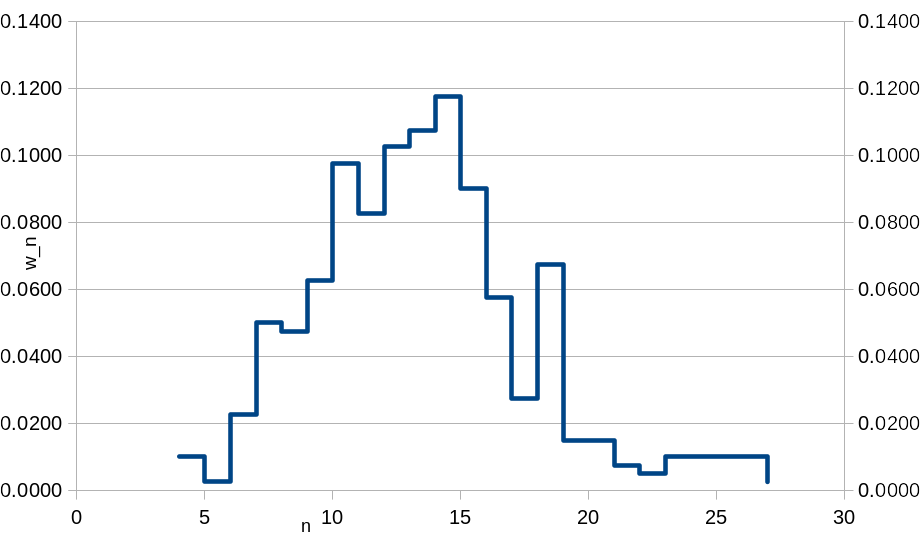
\includegraphics[scale = 0.4]{data/hist_10.png}
		\end{figure}

		Среднее значение для этой выборки $\overline{n}_1 = 14.1$, стандартное отклонение
		$\sigma_{\overline{n}_1} = 6.5$, относительная ошибка $\varepsilon_1 = 0.014$.

		\item Аналогичным образом обработаем данные для $\tau = 40$ с.
		\begin{table}[H]
			\centering
			\caption{Гистограмма для $\tau = 40$ с}
			\begin{tabular}{|c|c|c|}
				\hline
				Число импульсов $n$ & Число случаев & Доля случаев $\omega_n$ \\ \hline
				26                  & 1             & 0.0100                  \\ \hline
				32                  & 0             & 0.0025                  \\ \hline
				34                  & 2             & 0.0225                  \\ \hline
				36                  & 5             & 0.0500                  \\ \hline
				38                  & 5             & 0.0475                  \\ \hline
				40                  & 6             & 0.0625                  \\ \hline
				42                  & 10            & 0.0975                  \\ \hline
				44                  & 8             & 0.0825                  \\ \hline
				46                  & 10            & 0.0975                  \\ \hline
				48                  & 11            & 0.1125                  \\ \hline
				50                  & 12            & 0.1175                  \\ \hline
				52                  & 9             & 0.0900                  \\ \hline
				54                  & 6             & 0.0575                  \\ \hline
				56                  & 7             & 0.0675                  \\ \hline
				58                  & 1             & 0.0125                  \\ \hline
				60                  & 2             & 0.0150                  \\ \hline
				62                  & 2             & 0.0150                  \\ \hline
				64                  & 1             & 0.0075                  \\ \hline
				66                  & 2             & 0.0225                  \\ \hline
				76                  & 1             & 0.0050                  \\ \hline
				82                  & 1             & 0.0050                  \\ \hline
			\end{tabular}
		\end{table}

		\item Гистограмма по таблице 3:
		\begin{figure}[H]
			\centering
			\caption{Гистограмма для $\tau = 40$ с}
			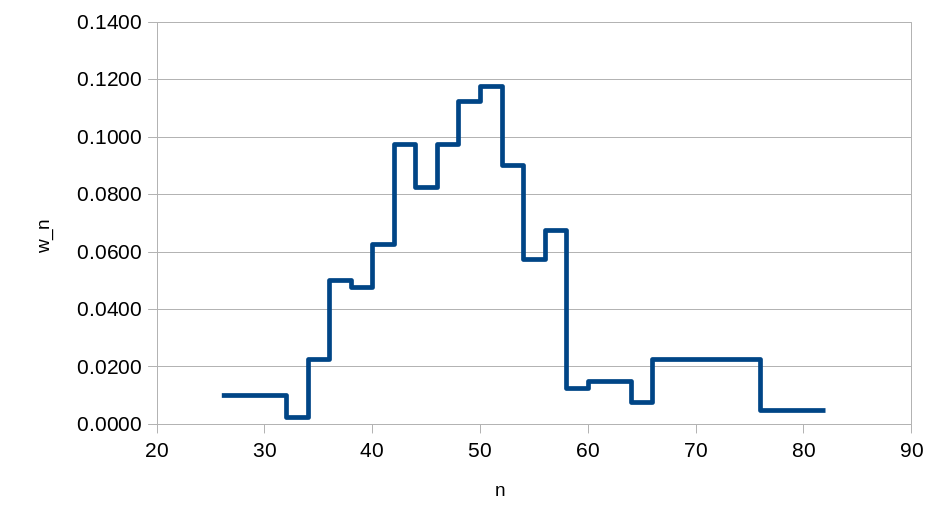
\includegraphics[scale = 0.4]{data/hist_20.png}
		\end{figure}

		Среднее значение $\overline{n}_2 = 50.7$, отклонение $\sigma_{\overline{n}_2} = 14.5$.
		Относительная ошибка $\varepsilon_2 = 0.015$.
	\end{enumerate}

	\section{Обсуждение результатов}
	Согласно теории, стандартное отклонение для распределения Пуассона можно
	оценить по формуле (1) как $\sigma = \sqrt{\overline{n}}$. Можно составить таблицу для
	этих опытов для сравнения результатов с теоретической оценкой:
	\begin{table}[H]
		\centering
		\caption{Стандартное отклонение для 2-х выборок}
		\begin{tabular}{|c|c|c|}
			\hline
			Выборка	& $\sigma_{\text{эксп}}$ & $\sigma_{\text{теор}}$ \\ \hline
			10 с    & 6.5                    & 3.8					  \\ \hline
			40 с	& 14.5					 & 7.1					  \\ \hline
		\end{tabular}
	\end{table}

	Нетрудно видеть, что порядок сходится с теоретической оценкой. Так же видна
	тенденция к уменьшению отклонения при увеличении числа измерений, что согласуется
	с теорией. Причиной существенного несовпадения значений с теорией могут быть
	некоторые радиационные аномалии, а также системная погрешность аппаратуры.

	\section{Вывод}
	В результате эксперимента удалось подтвердить характер распределения Пуассона, а также
	измерить средние значения.

\end{document}
